\chapter{Implementation}\label{ch:implementation}

\section{Output Switch Matrix Optimizations}\label{sec:osm}
\subsection{Description}
The different boards must route the data differently to the FEX systems depending on the detector region they are connected to. To tackle this problem, either each LATOME has a different version of the firmware, or some code must be added to allow an online configuration procedure defining the routing. The second possibility was chosen in the LAr group, and the solution proposed by Marcos for the V6 firmware was to add an Output Switch Matrix. 

The OSM uses multiplexers to route the 17 inputs to the 48 outputs and takes its selection bits from registers configured online via an ipbus. The HLS implementation is very simple, mainly involving a 2D array with 48 rows made of a subgroup of the 17 possible inputs.

\begin{figure}
    \centering
    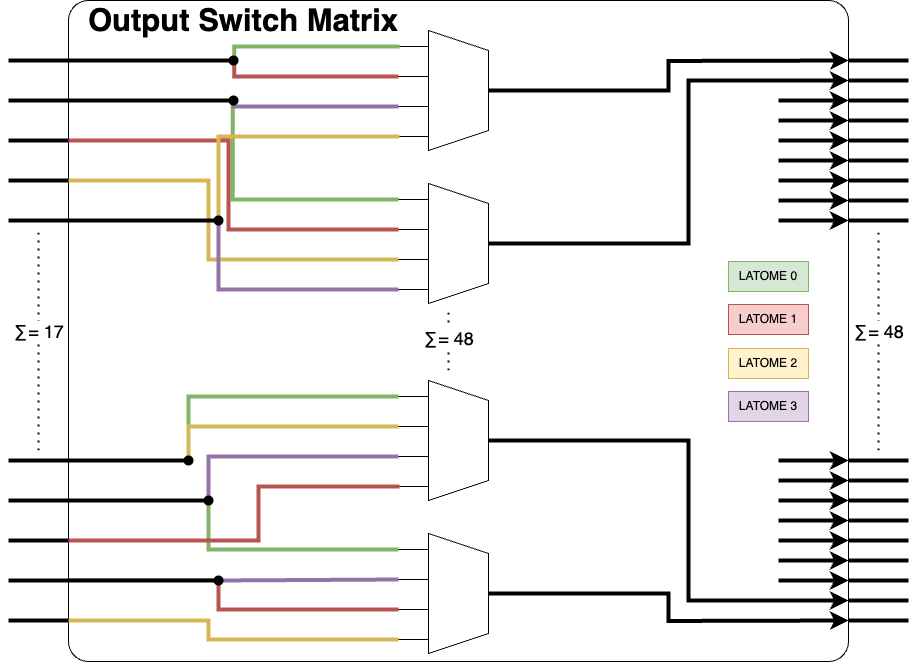
\includegraphics[width=0.6\textwidth]{osm.png}
    \caption{Output Switch Matrix Simplified Diagram}
    \label{fig:original-vhdl-design}
\end{figure}

Without looking at the different LATOME routings, it appears that, there should be 48 multiplexers of input size \(224\times17=3808\).
However when considering the data paths and optimizing for them, the biggest multiplexers have at most 4 input frames, meaning that each row from the HLS 2D array have 4 entries.
Figure \ref{fig:osum-v6} shows the parallel to serial block creating 32 bits words for the FEX systems. Moving this block to the left would have no impact on the latency. However, by moving this block before the Output Switch Matrix, the biggest multiplexers would have an input size of \(4\times32\) instead of \(4\times224\).

An important aspect to monitor is the data dependencies, since these could have a critical impact if using TDM. The OSM block is a routing block which does not change any data in the frames. The Frame Alignment only overwrites the data that it gets as input if the current BC index is an alignment one, hence it does not show data dependencies. Finally the Cyclic Redundant Check can be both computed in a parallel or serial fashion equivalently and only depends on the CRC temporary result from time \(t=-1\).

\subsection{Serializing Before the OSM}

Serializing the 224-bit full frames to 32-bit words requires 7 clock cycles, as \(224/7=32\). Hence the operating frequency of the OSUM block must be \(7\times40=280MHz\). The seven sequential cycles are created using a simple for loop without any catapult unroll directives. Instead of routing full frames, the OSM block now routes 32 bits words one at a time. Then the frame alignment and CRC9 blocks use a counter to keep track of the current word being processed. In the case of the CRC9, since the code is appended on the 9 last bits of the frames, the block must first compute 6 32-bit word followed by one 23-bit word. The overhead of having two specialized blocks is considered to be very small as each of them only contain a limited number of XOR gates.

\subsection{Improvements}
The expected results are an increase of the maximum operating frequency, as less signals must be synchronized, as well as an area reduction of a factor of 7.

\begin{table}[ht]
    \centering
    \begin{tabular}{|c|c|c|}
        \hline
        Version & Area (ALMs) & \(F_{max}\) (MHz) \\
        \hline
        Original OSM & 3621.5 & 310.17 \\
        Serialized OSM & 476.8 & 524.38  \\
        \hline
        Improvement & \(-86.8\%\) & \(+69.1\%\) \\
        \hline
    \end{tabular}
    \caption{Results From the OSM Optimization}
    \label{tab:osm-optimization}
\end{table}

The table \ref{tab:osm-optimization} shows an actual area reduction of a factor of 7.6 and an increase of the maximum operating frequency of 69\%. The area reduction is slightly higher than the expected factor of 7, which can be explained by the overhead that the signal synchronization logic had on the original design. 

\subsection{Serializing the Next Blocks}
As the figure \ref{fig:osum-v6} shows, the Frame Alignment and CRC9 blocks are two blocks that should be modified to handle the serial inputs.

\subsubsection{Frame Alignment}
The frame alignment block reads the current BC index and if it matches the alignment index, it overwrites the data with the new data, otherwise it simply forwards it. The introduction of a simple counter indicating which of the 7 words is currently being processed together with a ``switch'' statement taking care of the different cases is enough to get a TDM version of this block. Additionally, this block sends a 4 bit control character indicating for each byte if it is a data byte or a control byte. Before the serialization, the block would send the complete 28-bit control word, now it sends 4 bits at a time.

When developing the HLS code for these design blocks, two options can be considered using CCOREs, as illustrated in figure \ref{fig:unrolling-inside-outside}. The first one is to set the OSM, Frame Alignment or CRC9 as an elementary block processing only one frame at a time, and to create as many copies as there are frames to process. The second option is to make the design block process all the frames, and to set it as a CCORE. Using the HLS jargon, the first option refers to \textit{unrolling} ``outside'' of the CCORE, while the second refers to \textit{unrolling} ``inside'' of the CCORE.

\begin{figure}
    \centering
    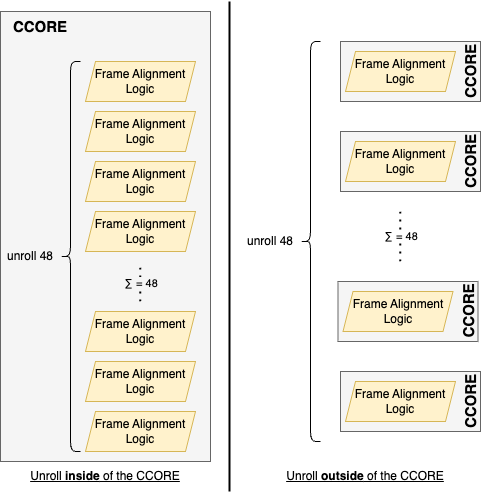
\includegraphics[width=0.6\textwidth]{unroll_inside_outside.png}
    \caption{Unrolling inside vs outside the CCORE}
    \label{fig:unrolling-inside-outside}
\end{figure}

In the case of the Frame Alignment, the V6 firmware uses the first option. One frame alignment CCORE uses very little area, and because it uses only combinational logic, using the second option does not have any significant impact on the area. In table \ref{tab:frame-alignment-optimization}, we see that with the first option yields a Frame Alignment of 21 ALMs. To compare it with the second option, we can multiply it by the number of instances that will be created: 48, for the 48 frames. This gives a total area of 1008, very similar to the 1087 of the second option. The \(F_{max}\) parameter, on the other hand, decreases by 98MHz, but this should be disregarded as the ``unrolling inside'' version of the CCORE contains the logic to synchronize the different instances.

To have an idea of the true impact that the two implementation could have on the full firmware, the table \ref{tab:frame-alignment-optimization} also shows the area and \(F_{max}\) of the OSUM parent block. The low impact on the area is confirmed by our results, but the \(F_{max}\) gets a decrease of 3.6\%, reducing the margin of the design.

\begin{table}[ht]
    \centering
    \begin{tabular}{|c|c|c|}
        \hline
        \hline
        \multicolumn{3}{|c|}{unroll outside} \\
        \hline
        Block & Area (ALMs) & \(F_{max}\) (MHz) \\
        \hline
        Frame Alignment & \underline{21} (\(21\times48=1008\)) & 371.4 \\
        OSUM & 30449 & 274.5 \\
        \hline
        \hline
        \multicolumn{3}{|c|}{unroll inside} \\
        \hline
        Block & Area (ALMs) & \(F_{max}\) (MHz) \\
        \hline
        Frame Alignment & \underline{1087} (\(1087/48=22.6\))& 272.6\\
        OSUM & 30512 & 264.6\\
        \hline
    \end{tabular}
    \caption{Frame Alignment design exploration using the V6 firmware}
    \label{tab:frame-alignment-optimization}
\end{table}

In fact, using the second option can be useful in case some sequential logic could be shared among all the CCOREs. The serialized Frame Alignment is a good example where unrolling outside has a positive impact, as it can be seen in the table \ref{tab:new-frame-alignment-optimization}. In this specific case, Catapult is able to optimize the design inside of the CCORE by sharing some logic between the different parallel instances. As a result, unrolling inside of the CCORE will create redundant logic and the total area of the CCORE instances is almost the double of the ``unrolling inside'' version. Additionally, this negative impact gets amplified on the OSUM block, with an area increase of 15\% and new timing violations with the ``unroll outside'' option.

\begin{table}[ht]
    \centering
    \begin{tabular}{|c|c|c|}
        \hline
        \hline
        \multicolumn{3}{|c|}{unroll outside} \\
        \hline
        Block & Area (ALMs) & \(F_{max}\) (MHz) \\
        \hline
        Frame Alignment & \underline{36} (\(36\times48=1728\)) & 388.8 \\
        OSUM & 18669 & \(274.7 < 280\) \\
        \hline
        \hline
        \multicolumn{3}{|c|}{unroll inside} \\
        \hline
        Block & Area (ALMs) & \(F_{max}\) (MHz) \\
        \hline
        Frame Alignment & \underline{940} (\(940/48=19.6\))& 345.1\\
        OSUM & 15875 & 291.1\\
        \hline
    \end{tabular}
    \caption{Frame Alignment design exploration using the new firmware}
    \label{tab:new-frame-alignment-optimization}
\end{table}

\subsubsection{CRC9}

\section{Optimizing the HLS Directives}
